\section{Experiment}
To test localization accuracy, an one meter by one meter grid was set up and the arrays are placed at the top left and top right corners of the grid. Fig~\ref{fig:setup_point} shows a picture of the setup. 

\begin{figure}[]
  \centering
  \begin{subfigure}[]{.2\textwidth}
    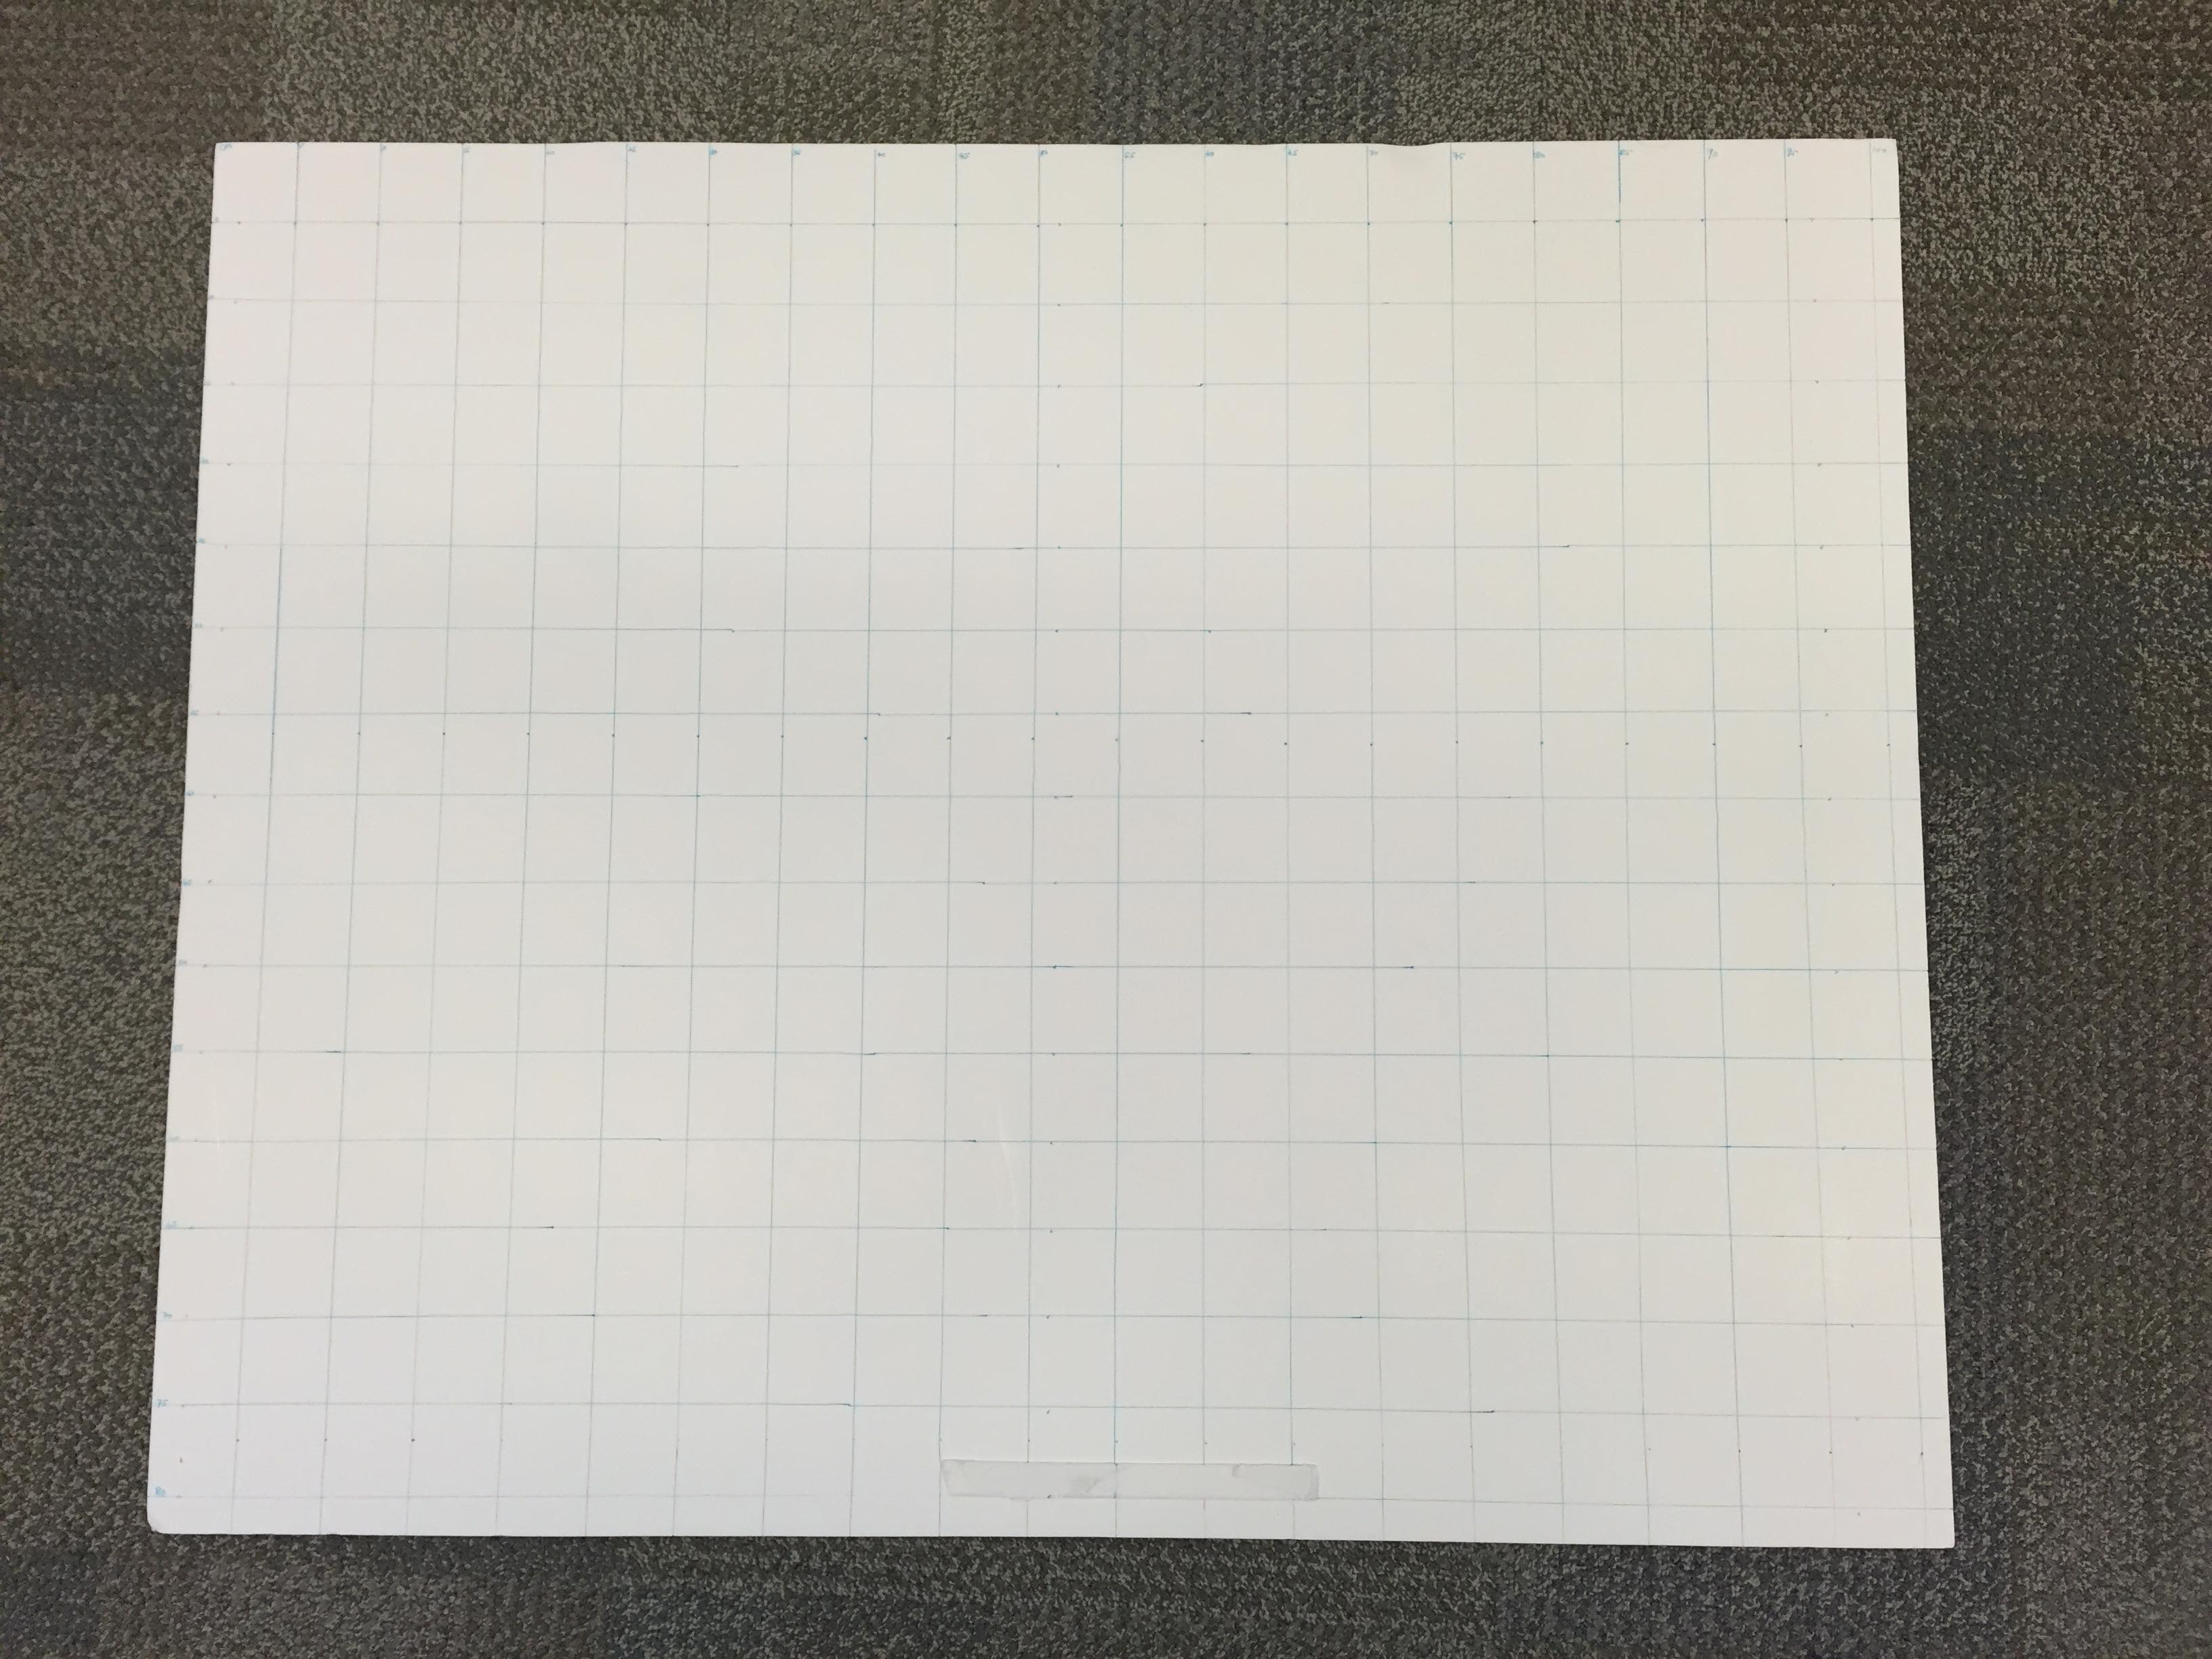
\includegraphics[width=\textwidth]{setup_1.JPG}
    \caption{1 meter by 1 meter grid}
  \end{subfigure}
  \begin{subfigure}[]{.2\textwidth}
    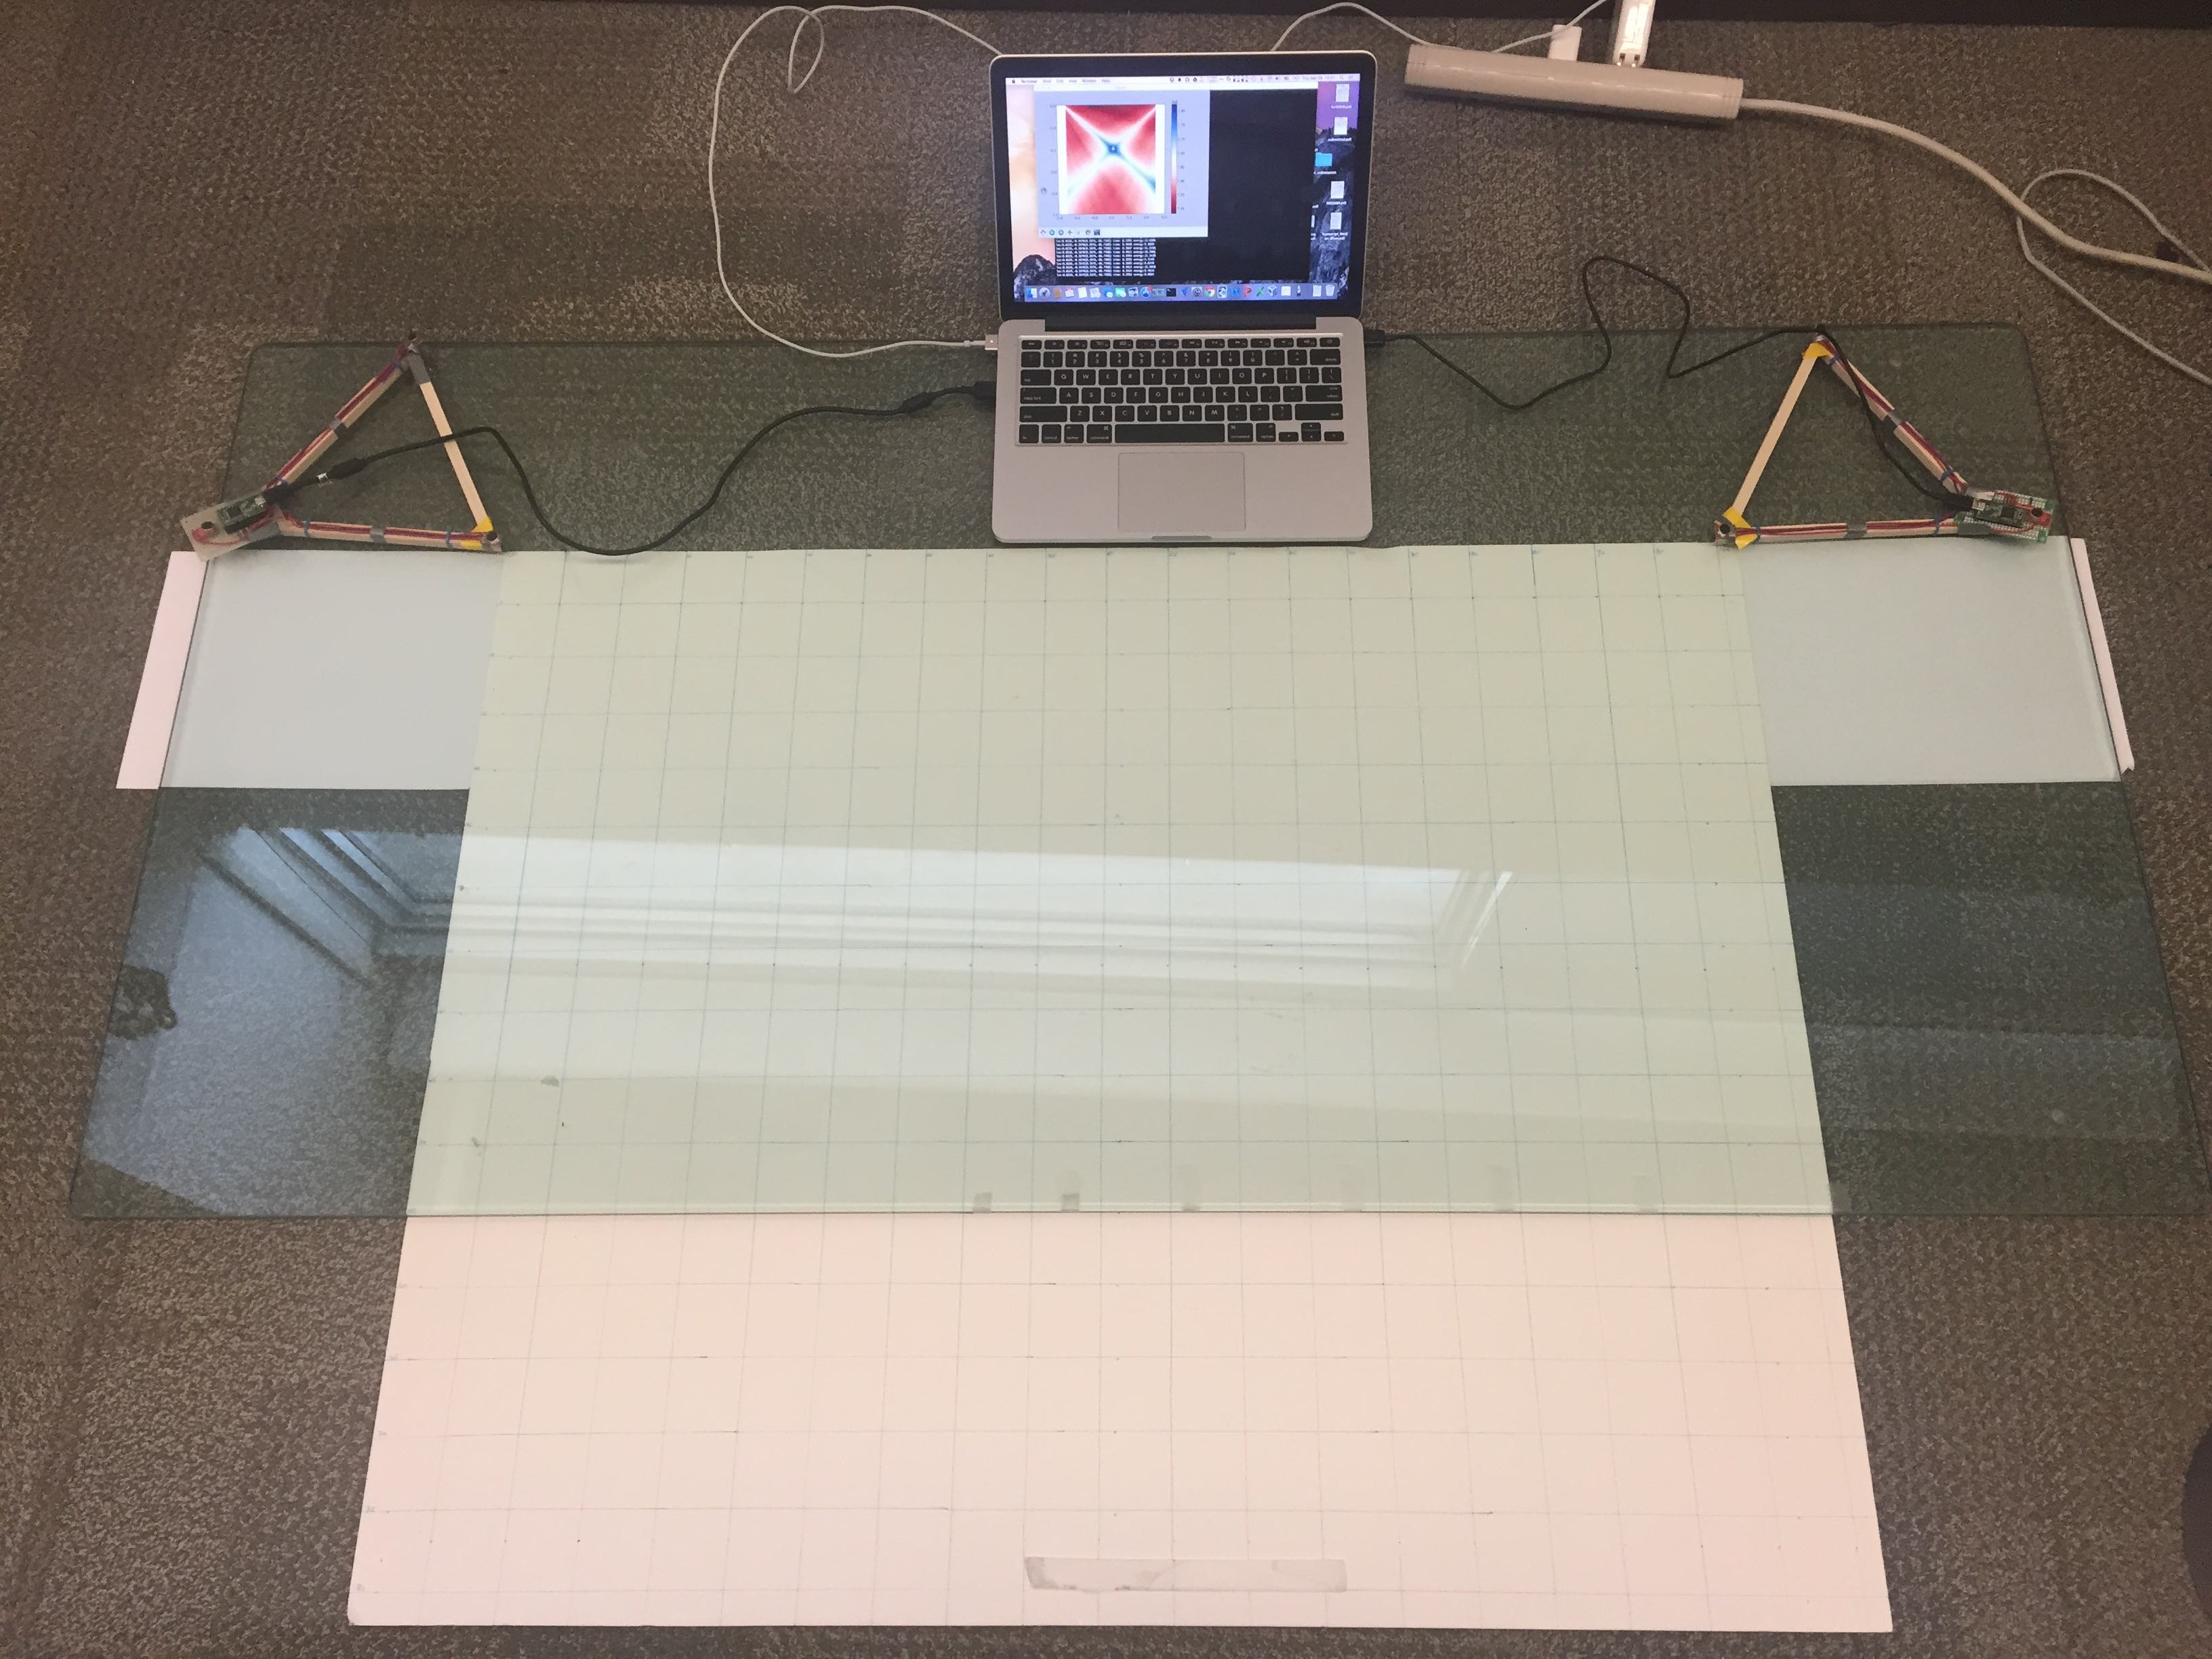
\includegraphics[width=\textwidth]{setup_2.JPG}
    \caption{array placement}
  \end{subfigure}
  \caption{Setup for localization accuracy testing}
  \label{fig:setup_point}
\end{figure}

A total of $32$ positions are chosen uniformly in this region where microphone data is recorded. To test how accuracy varies with window size, the algorithm is fed with recorded microphone data with different segment length. Fig~\ref{fig:accuracy_vs_window} shows how accuracy changes with window length for three GCC algorithms. The error lowers as window size increases and plataeus after window size exceeds around $10$ milli-second. The lowest error achieved is $2.53$ centimeters. It is achieved when window size is set to 12 millisecond and GCC\_PHAT is used to estimate difference of delay

Although accuracy improves with window length, the calculation time also increases with window length. The part of calculation that depends on window length is using cross correlation to estimate difference of arrival time. cross correlation can be calculated with FFT and the runtime is of order $O(N\log N)$. We measured how the computation time varies with window length and Figure~\ref{fig:speed_vs_window} shows the result. The runtime increases approximately linearly in the window size region of interest.

We also calculated the localization error for each tested point in the region. Figure~\ref{fig:error_distribution} shows a heatmap of the error distribution inside the grid. The error is below $3$ cm for most areas inside the region. There is one error spike in the mid-left region and we contribute this to audio source placecment error becuase the error is fairly low and consistent around that spike region.

\begin{figure}[]
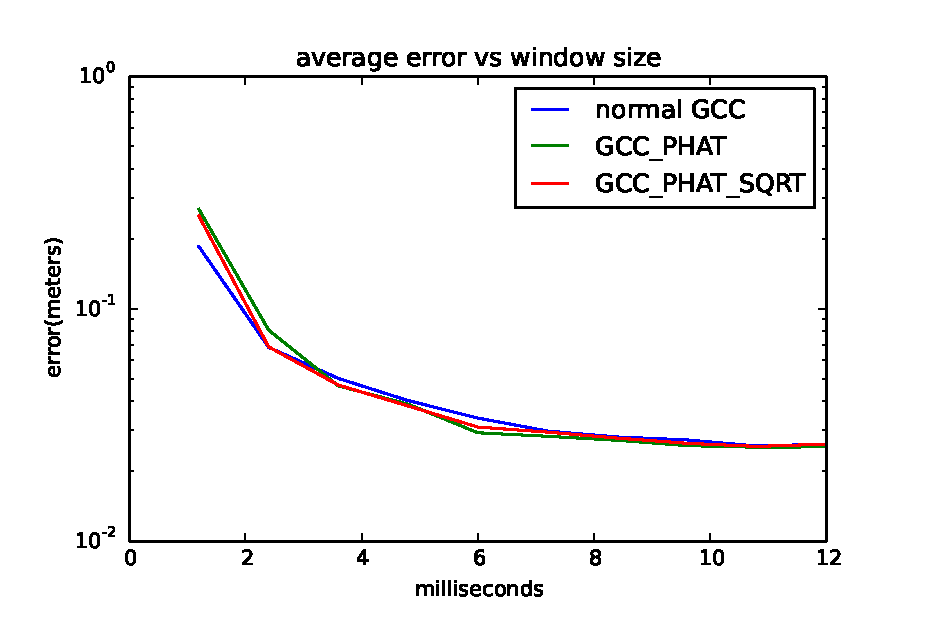
\includegraphics[width=0.5\textwidth]{average_error_window_size.eps}
\caption{accuracy versus window size}
\label{fig:accuracy_vs_window}
\end{figure}

\begin{figure}[]
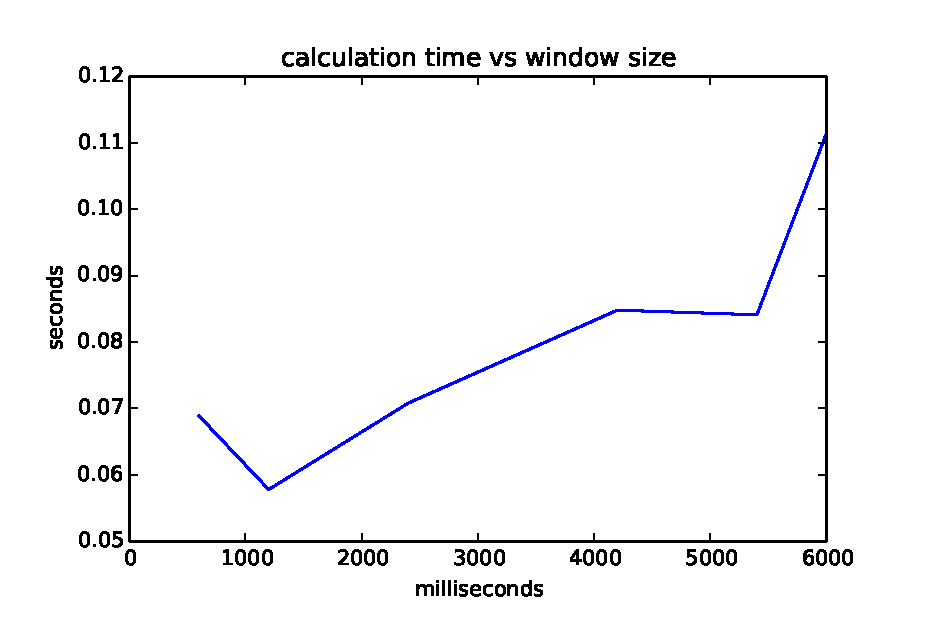
\includegraphics[width=0.5\textwidth]{calculation_time.eps}
\caption{speed versus window size}
\label{fig:speed_vs_window}
\end{figure}


\begin{figure}[]
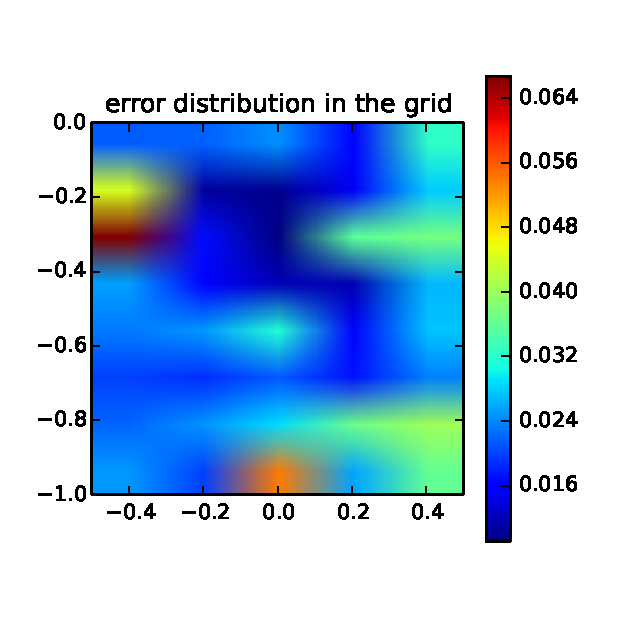
\includegraphics[width=0.5\textwidth]{error_distribution.eps}
\caption{error distribution in the grid}
\label{fig:error_distribution}
\end{figure}

\begin{figure}[]
  \centering
  \begin{subfigure}[]{.2\textwidth}
    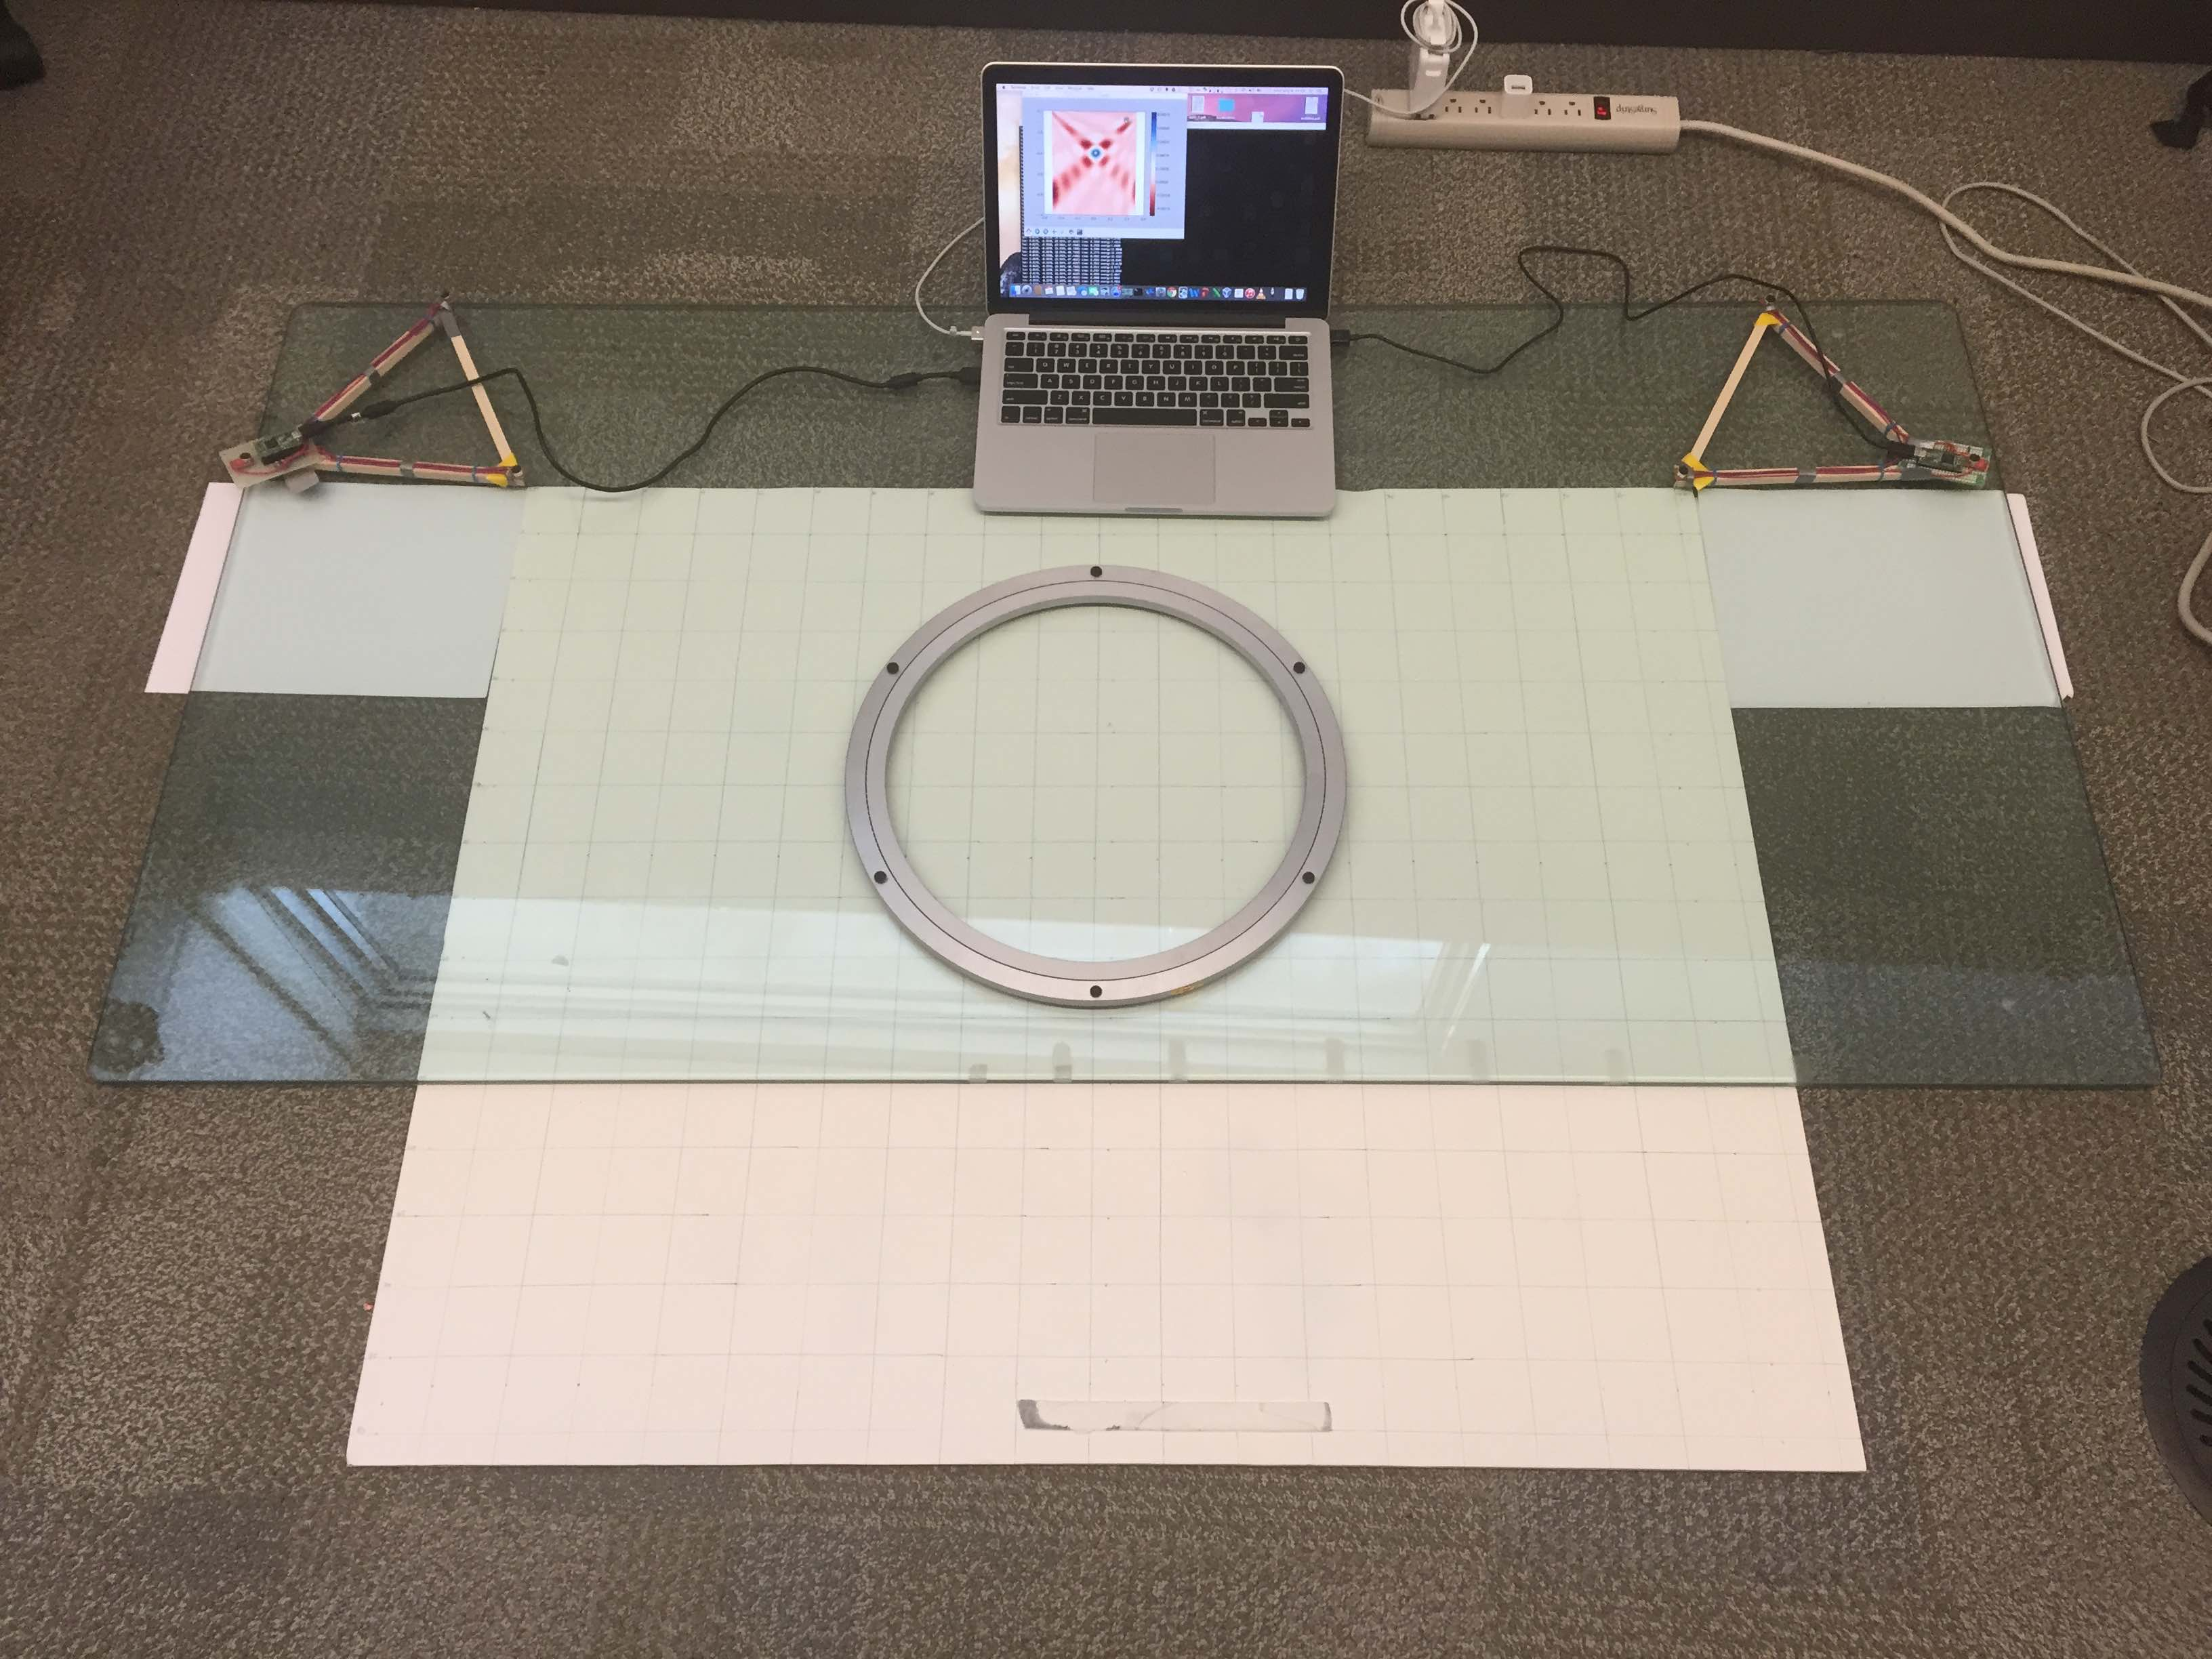
\includegraphics[width=\textwidth]{setup_ring.JPG}
  \end{subfigure}
  \begin{subfigure}[]{.2\textwidth}
    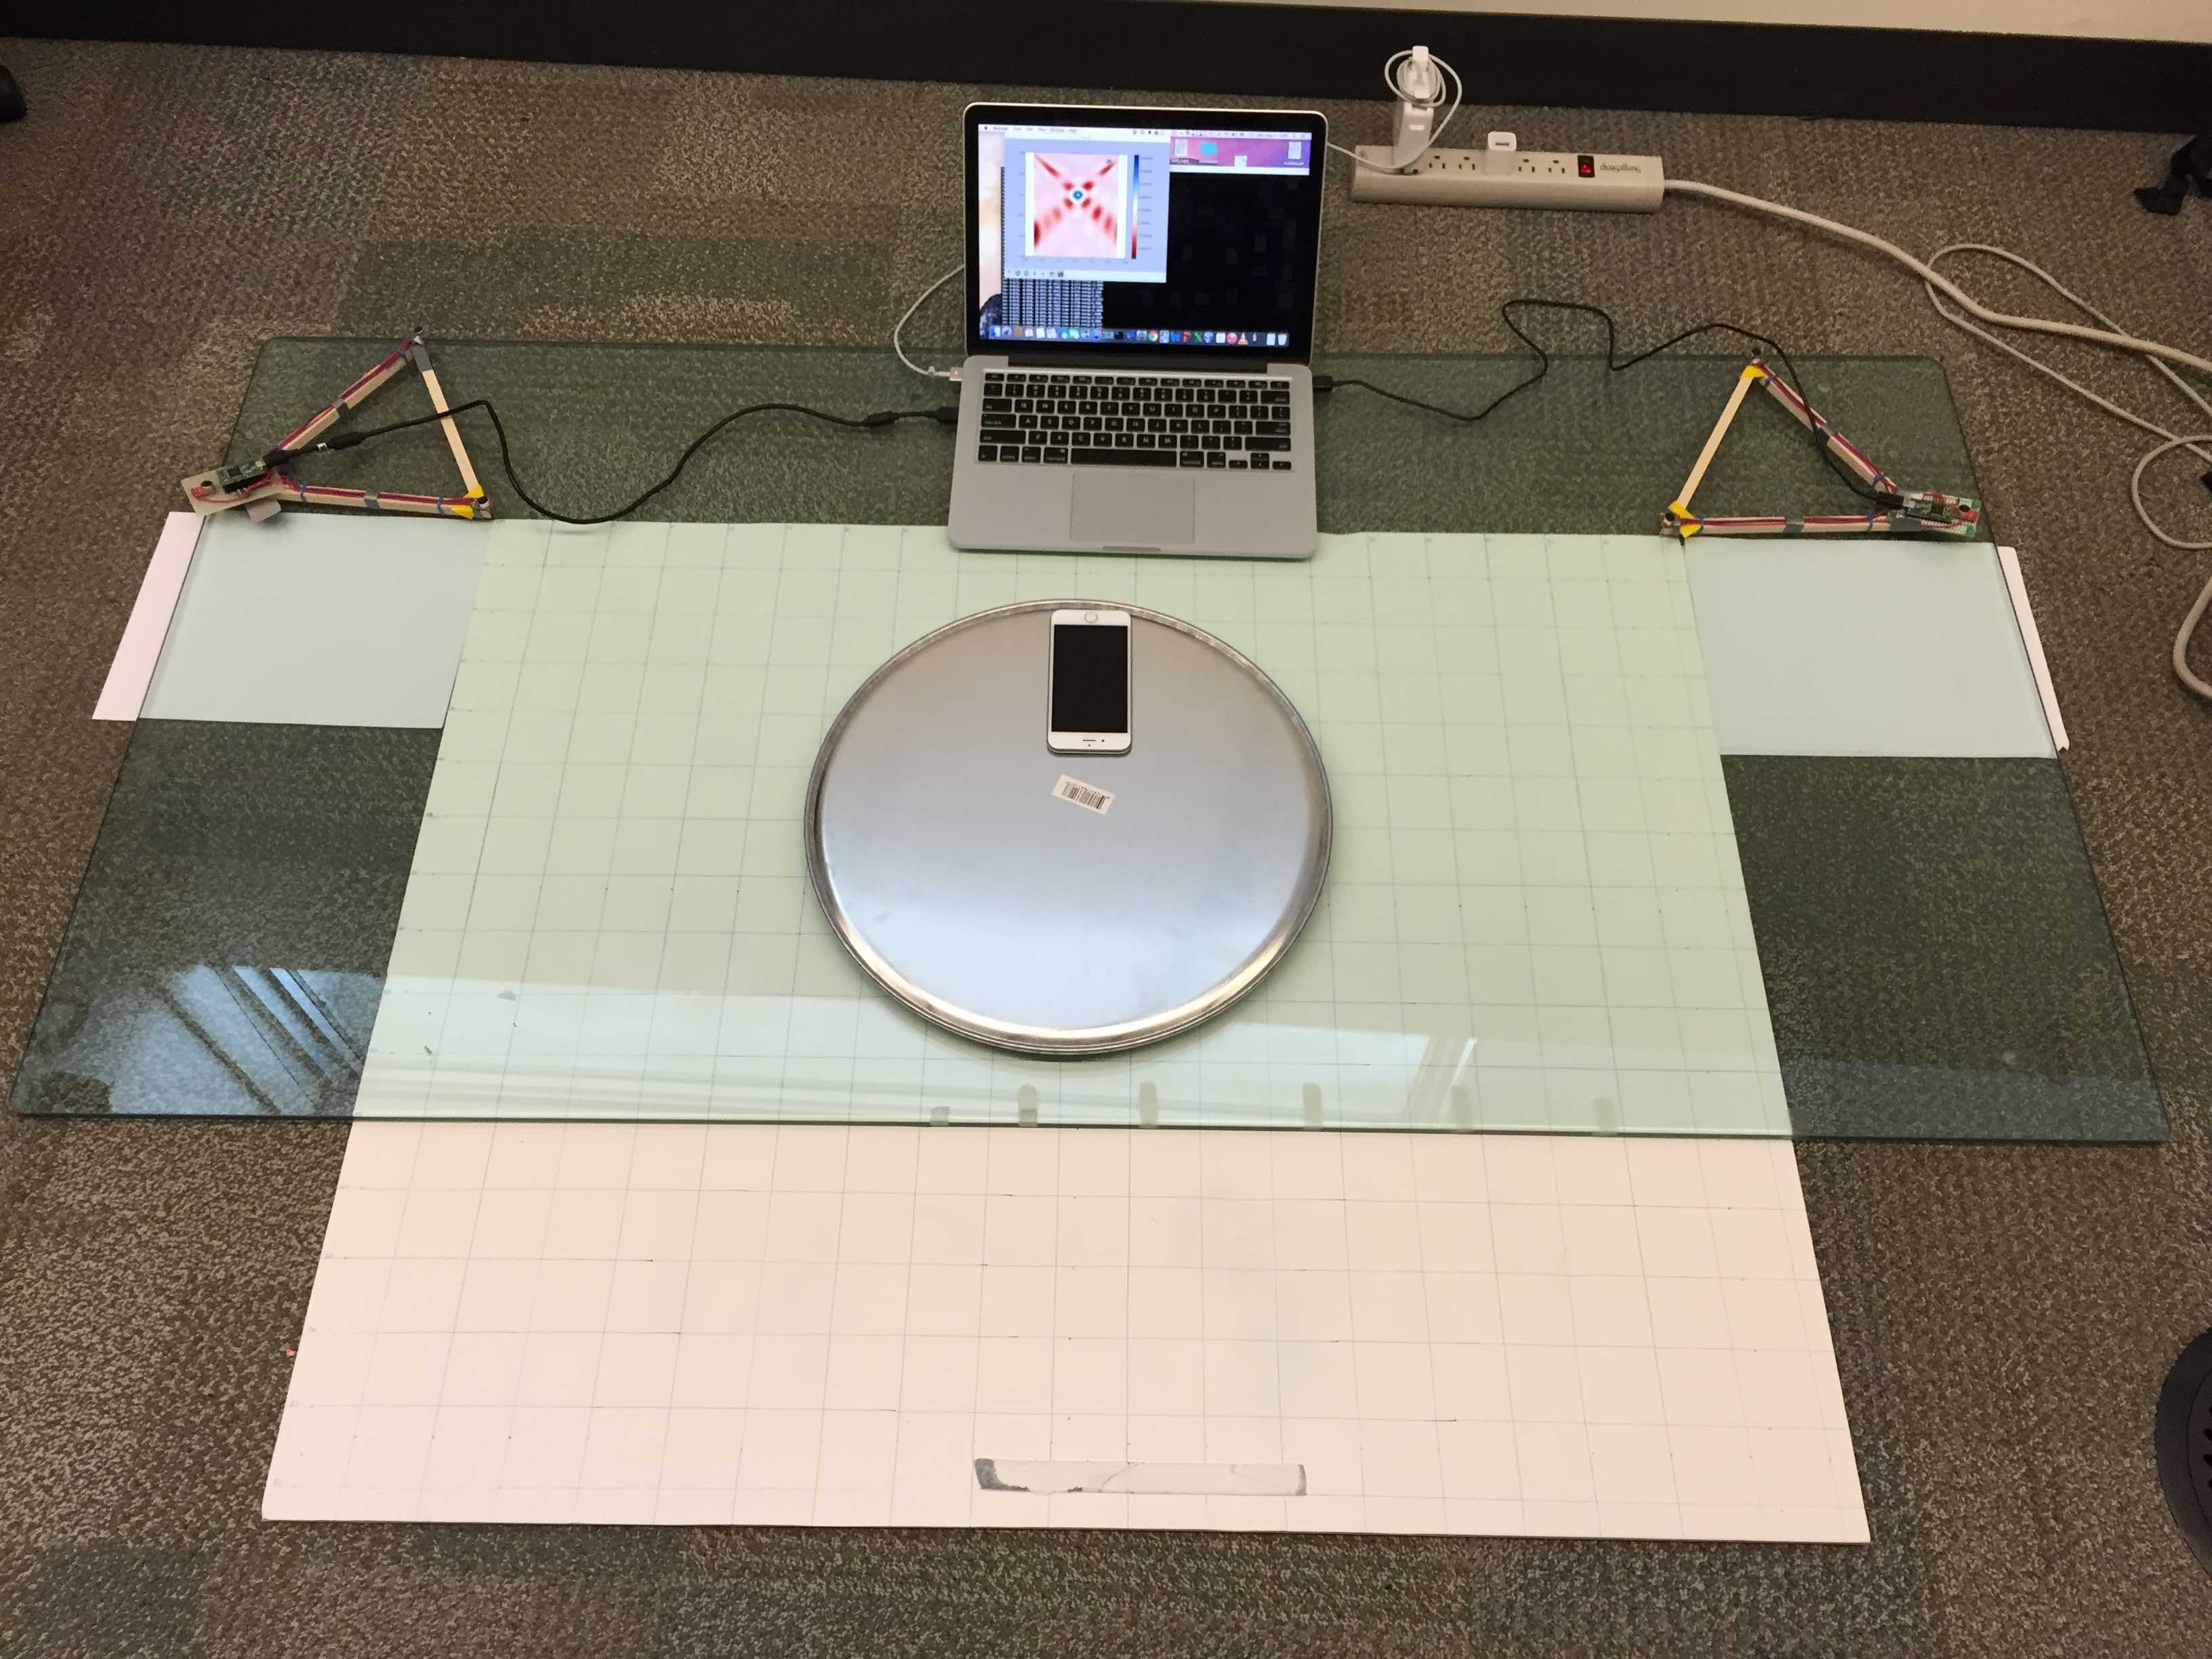
\includegraphics[width=\textwidth]{setup_rotating_disk.JPG}
  \end{subfigure}
  \caption{Setup for circle movement localization}
  \label{fig:setup_circle}
\end{figure}


To test how well the arrays track movement, we mounted a rotating disk $40$ centimeter in diameter onto the grid at $(x=0, y=-0.3)$. Fig~\ref{fig:setup_circle} shows a picture of the sestup. A sound source is placed on the edge of rotating disk and the arrays localizes the sound source as it rotates in a circle. In this experiment, we want to test how accuracy changes with:
\begin{itemize}
\item different window sizes
\item different audio sources
\item different movement tracking filters
\item different movement speeds
\end{itemize}


\begin{figure*}[]
\centering
  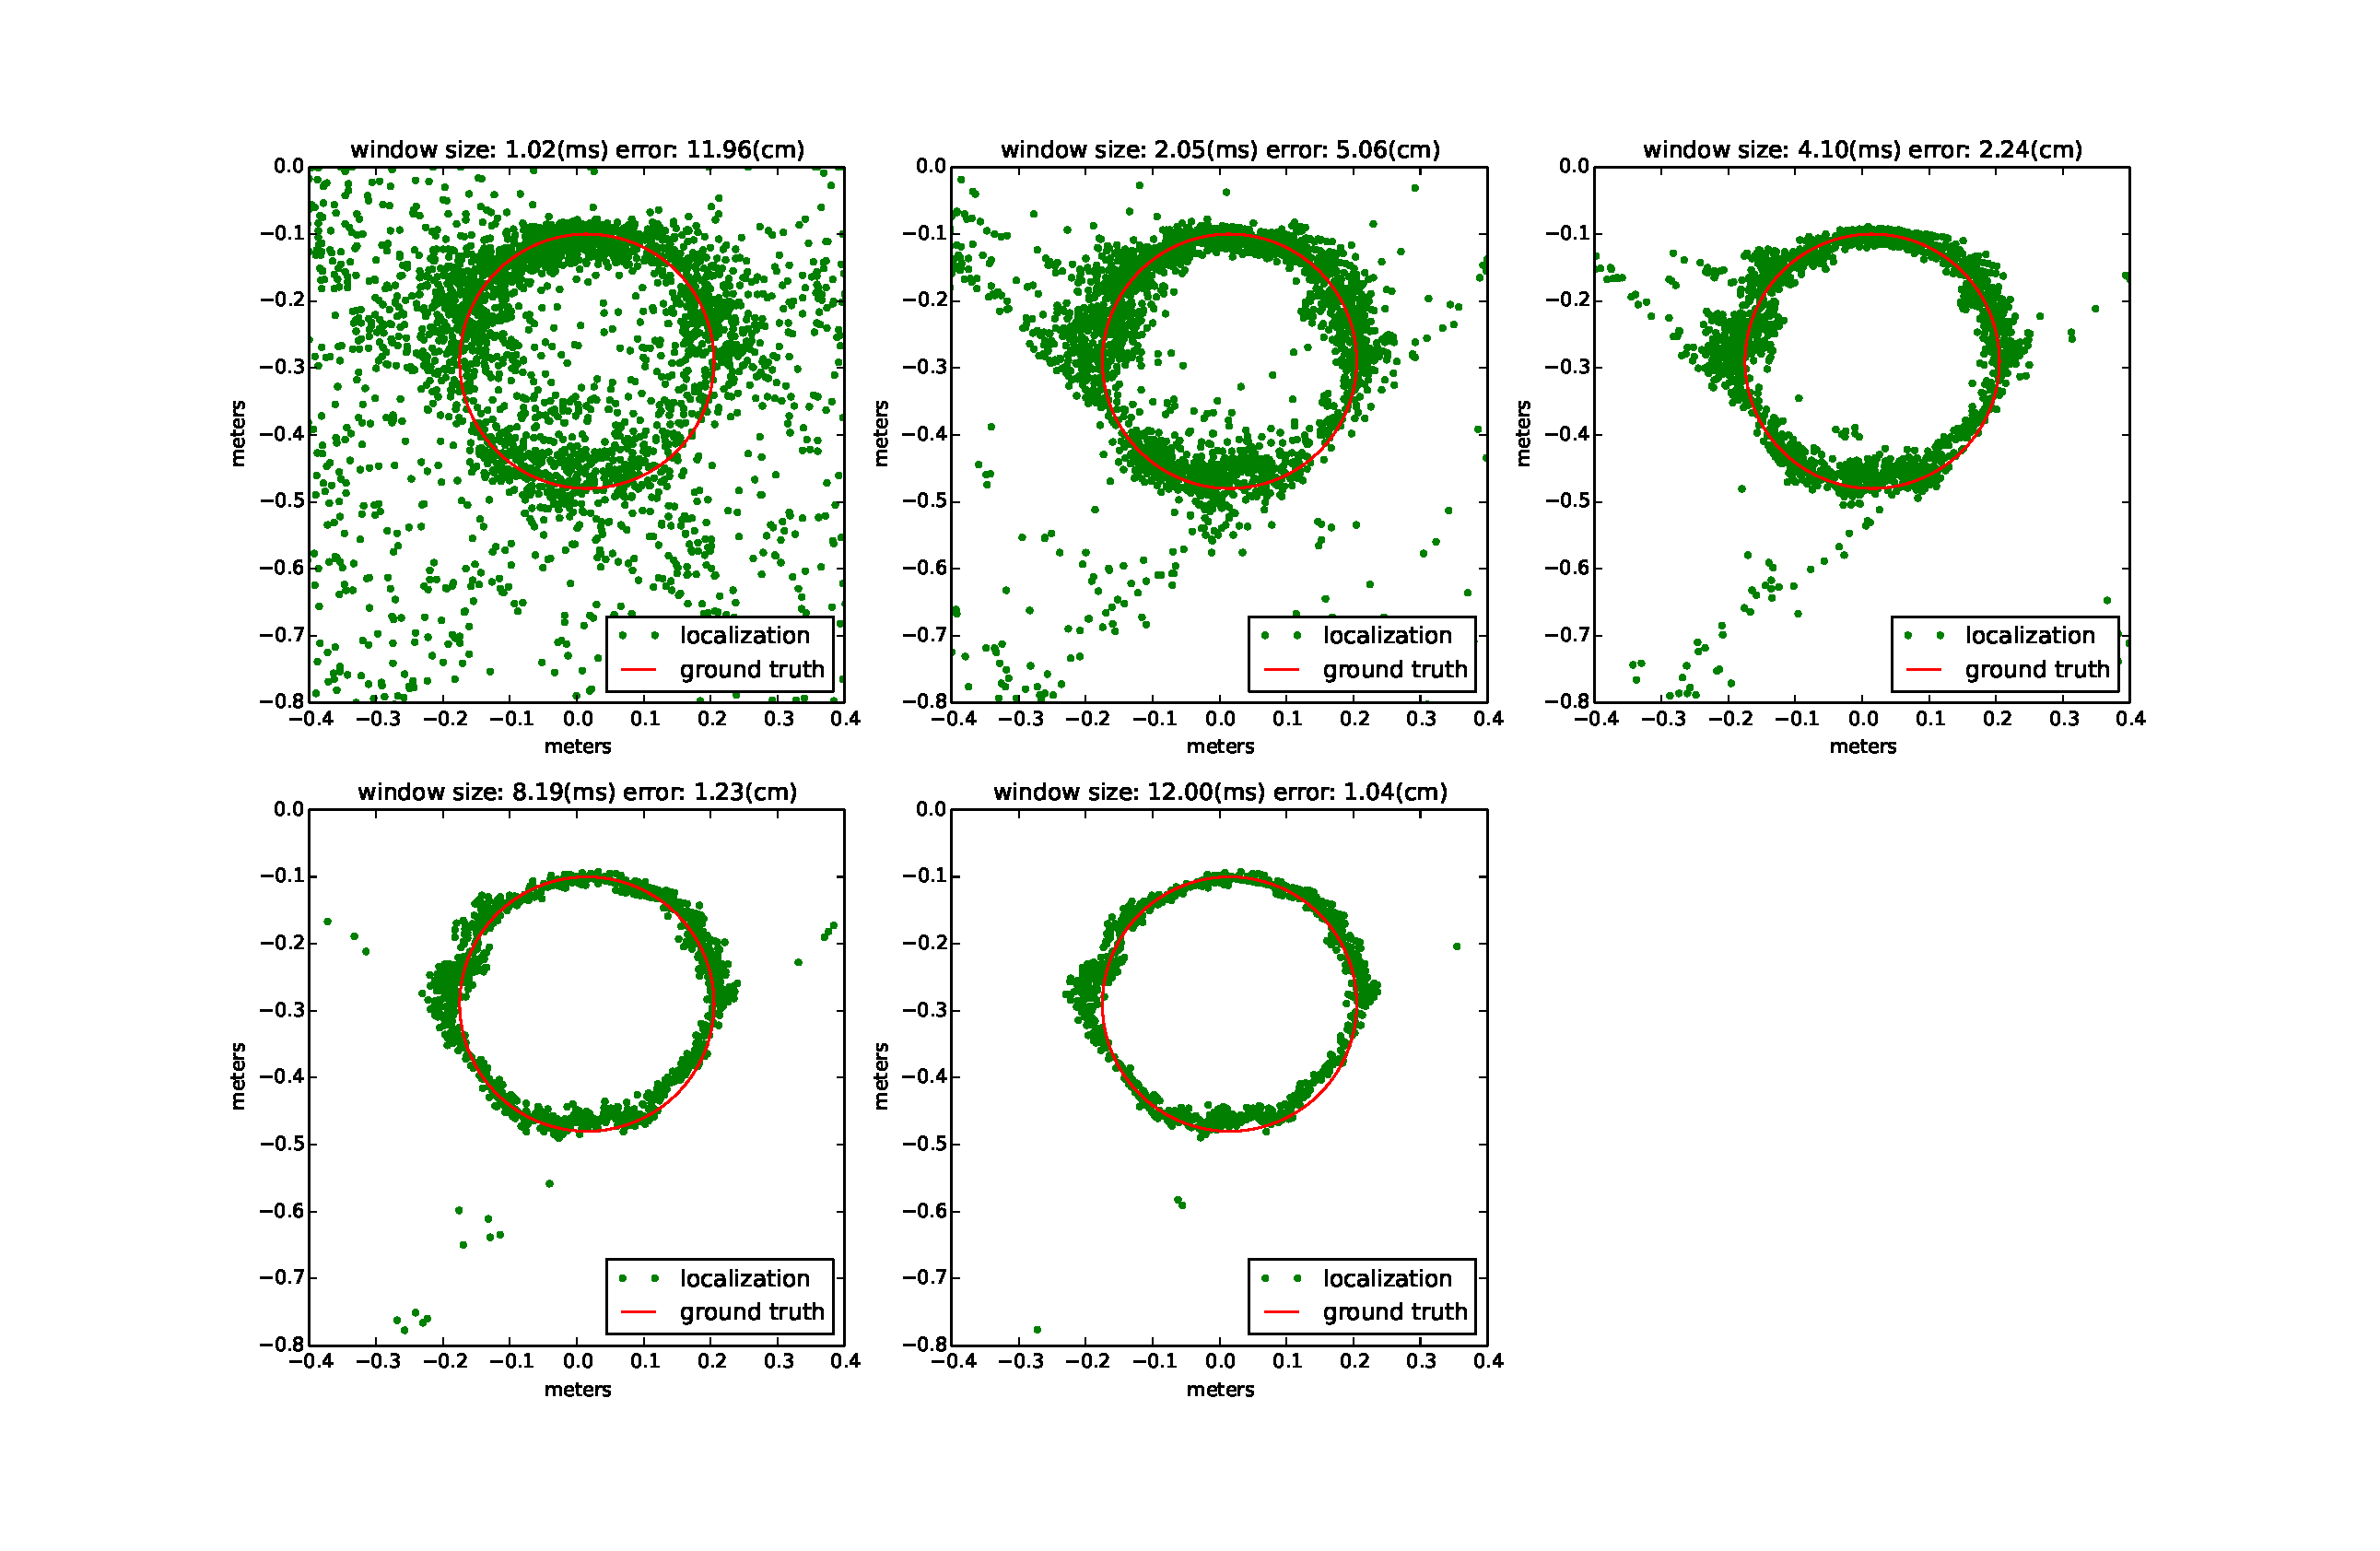
\includegraphics[width=\textwidth]{trace_window_size_movement.eps}
\caption{Localization quality versus window size}\label{fig:wn}
\label{fig:trace_win_circle}
\end{figure*}

\begin{figure}[]
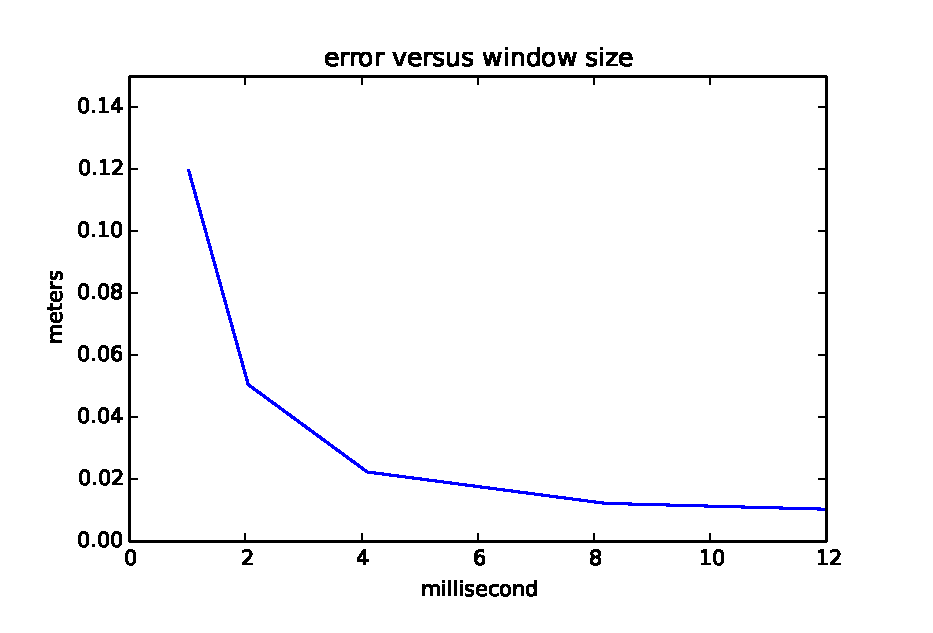
\includegraphics[width=0.5\textwidth]{error_window_size_movement.eps}
\caption{Localization error versus window size}
\label{fig:err_win_circle}
\end{figure}


Fig~\ref{fig:err_win_circle} gives an intuitive representation of how accuracy changes with window size. When window size is small($1.02$ millisecond), the audio does not contain enough information to reliably estimate arrival time differences. The localization is very noisy. As window size increases, the localization converges to the shape of ground truth circle. Fig~\ref{fig:err_win_circle} shows how the error changes with window size. The general trend is similar to that in point localization case. The error decreases as window size increases and plateaus after window size exceeds around $10$ milliseconds.

To test how different sound sources impact localization quality, three experiments on the same movement track were conducted with three different sound sources:

\begin{description}

\item[White Noise] A recording of white noise.

\item[Music A] A music that has normal audio amplitude throughout experiment period was chosen. "Honest Eyes" by Black Tide was chosen 

\item[Music B] A music with intermittent low amplitude sections was chosen. "Canon" was used.

\end{description} 

To test how audio movement source affects localization quality, each of three experiments were conducted at two different speeds:
\begin{description}
\item[Normal] An angular speed of $0.5$ rad/s was maintained, which translates to linear speed of $10$ cm/s.
\item[Fast] An angular speed of $1.0$ rad/s was maintained, which translates to linear speed of $20$ cm/s.
\end{description}

For each experiment conducted, two different movement filters are tests:
\begin{description}
\item[Averaging filter] localization for past $0.5$ seconds are averaged and outputed as current estimate.
\item[Kalman filter] A 2nd order Kalman filtering is used.
\end{description}

\begin{figure*}[]
\centering
\begin{subfigure}[]{1.0\textwidth}
  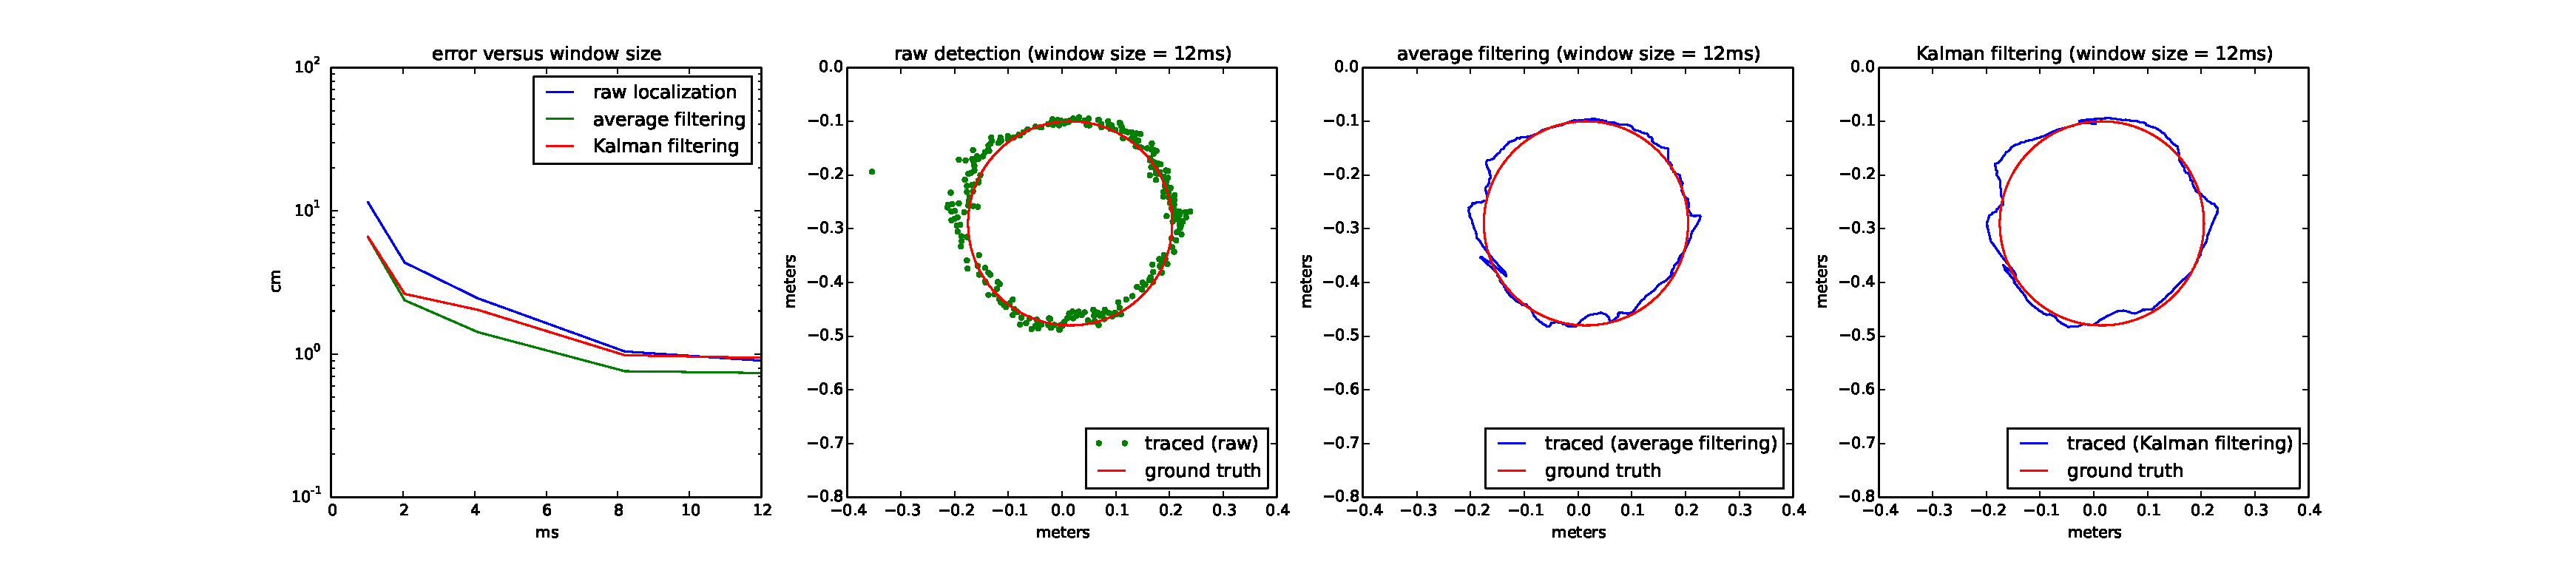
\includegraphics[width=1.0\textwidth]{trace_output_circle_wnn.eps}
  \caption{white noise}
  \label{fig:circle_wn}
\end{subfigure}
\begin{subfigure}[]{1.0\textwidth}
  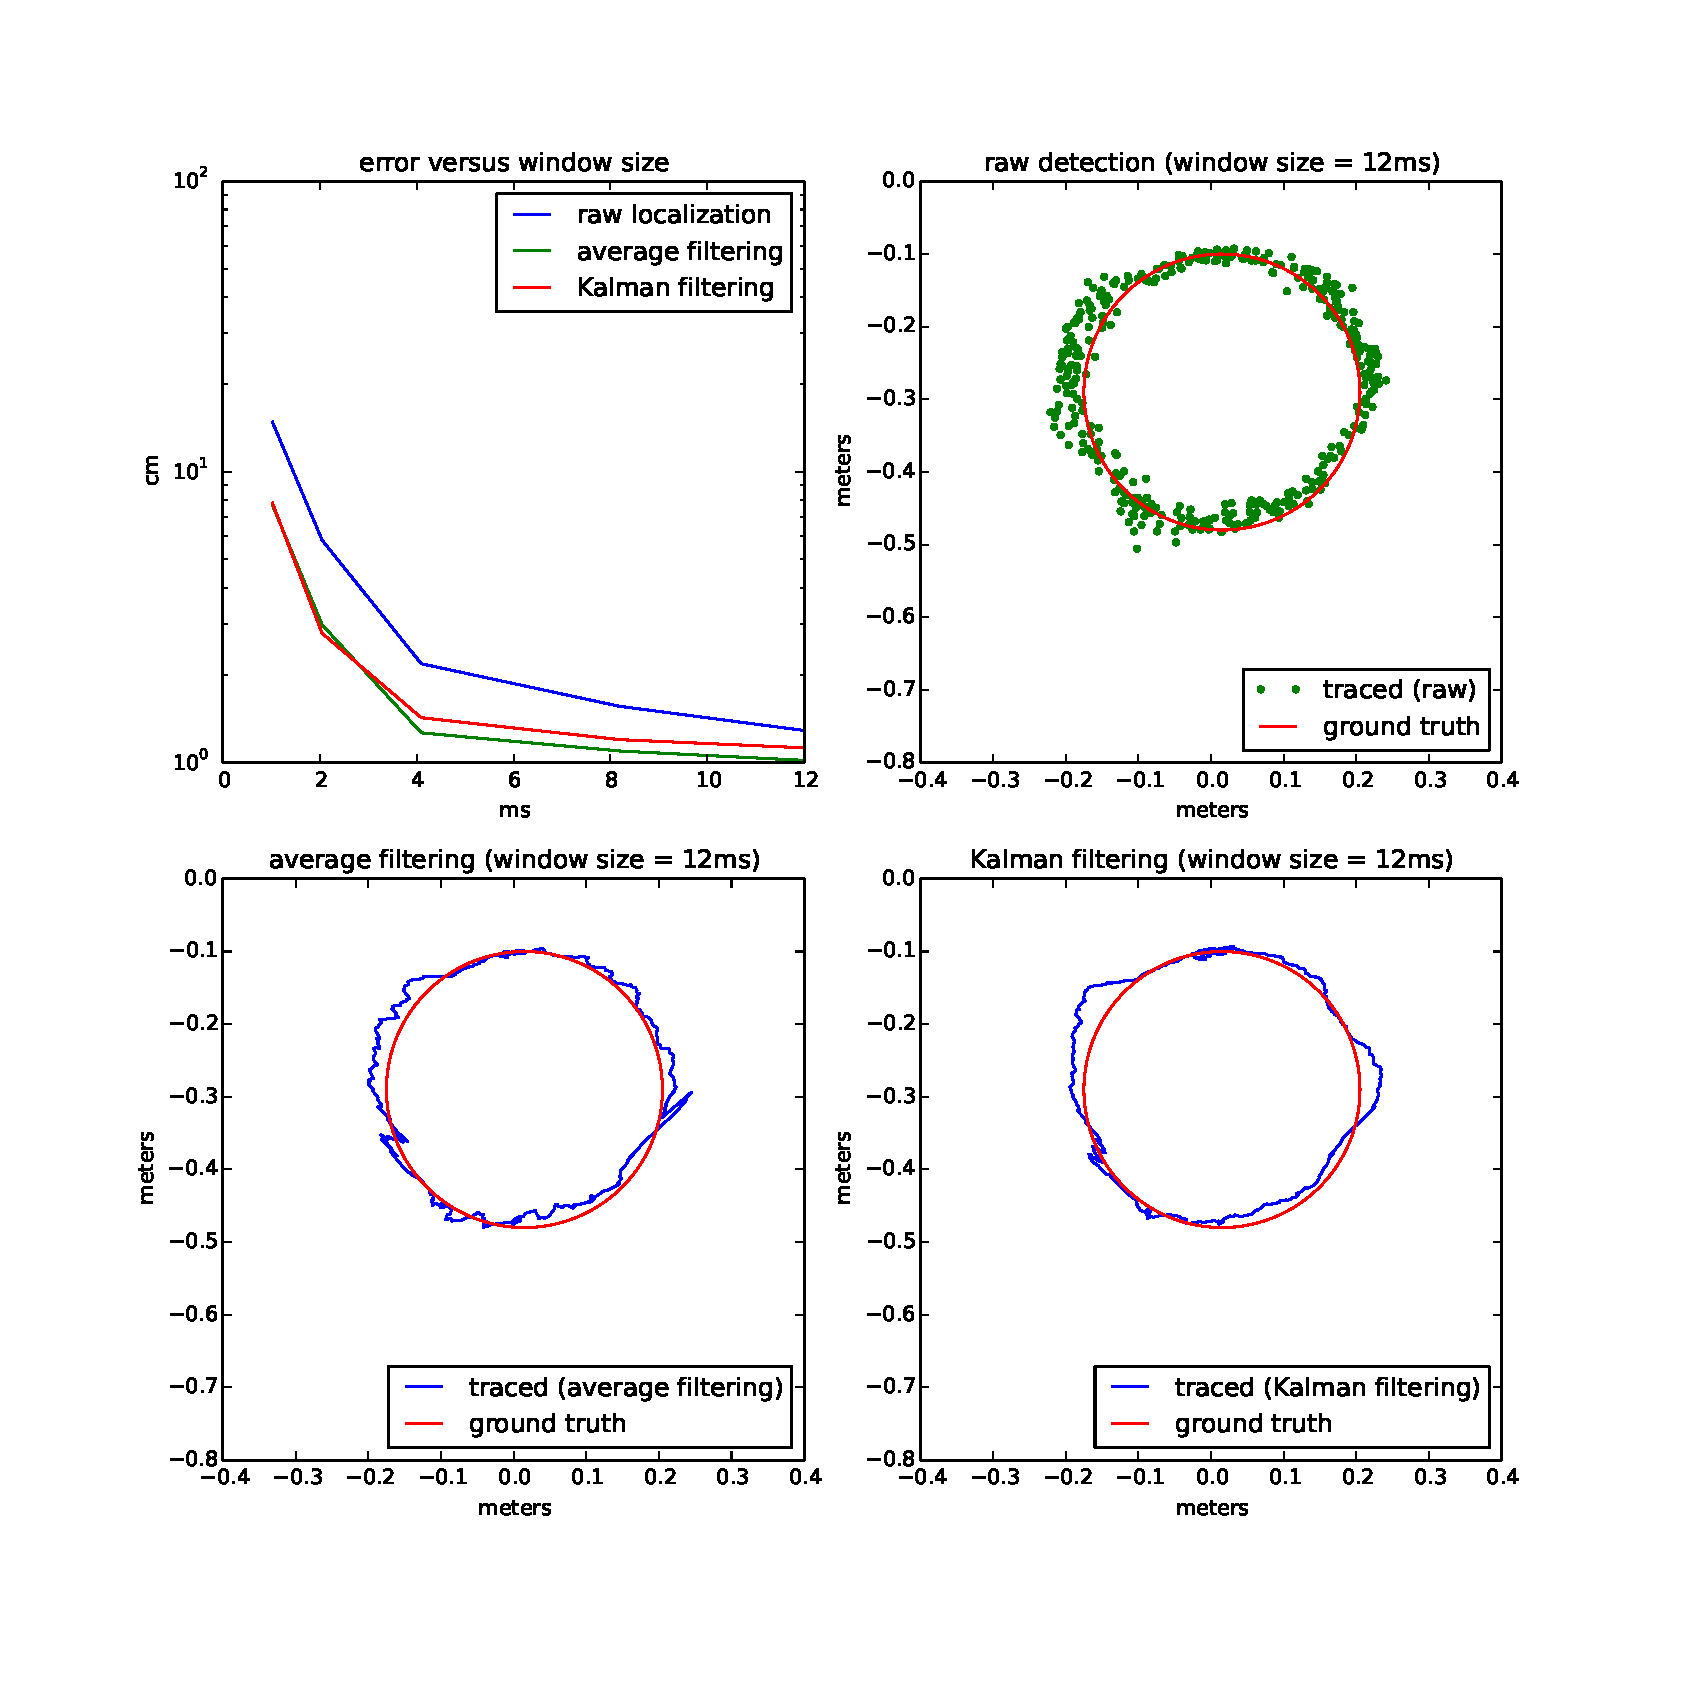
\includegraphics[width=\textwidth]{trace_output_circle_man.eps}
  \caption{music A}
  \label{fig:circle_musica}
\end{subfigure}
\begin{subfigure}[]{1.0\textwidth}
  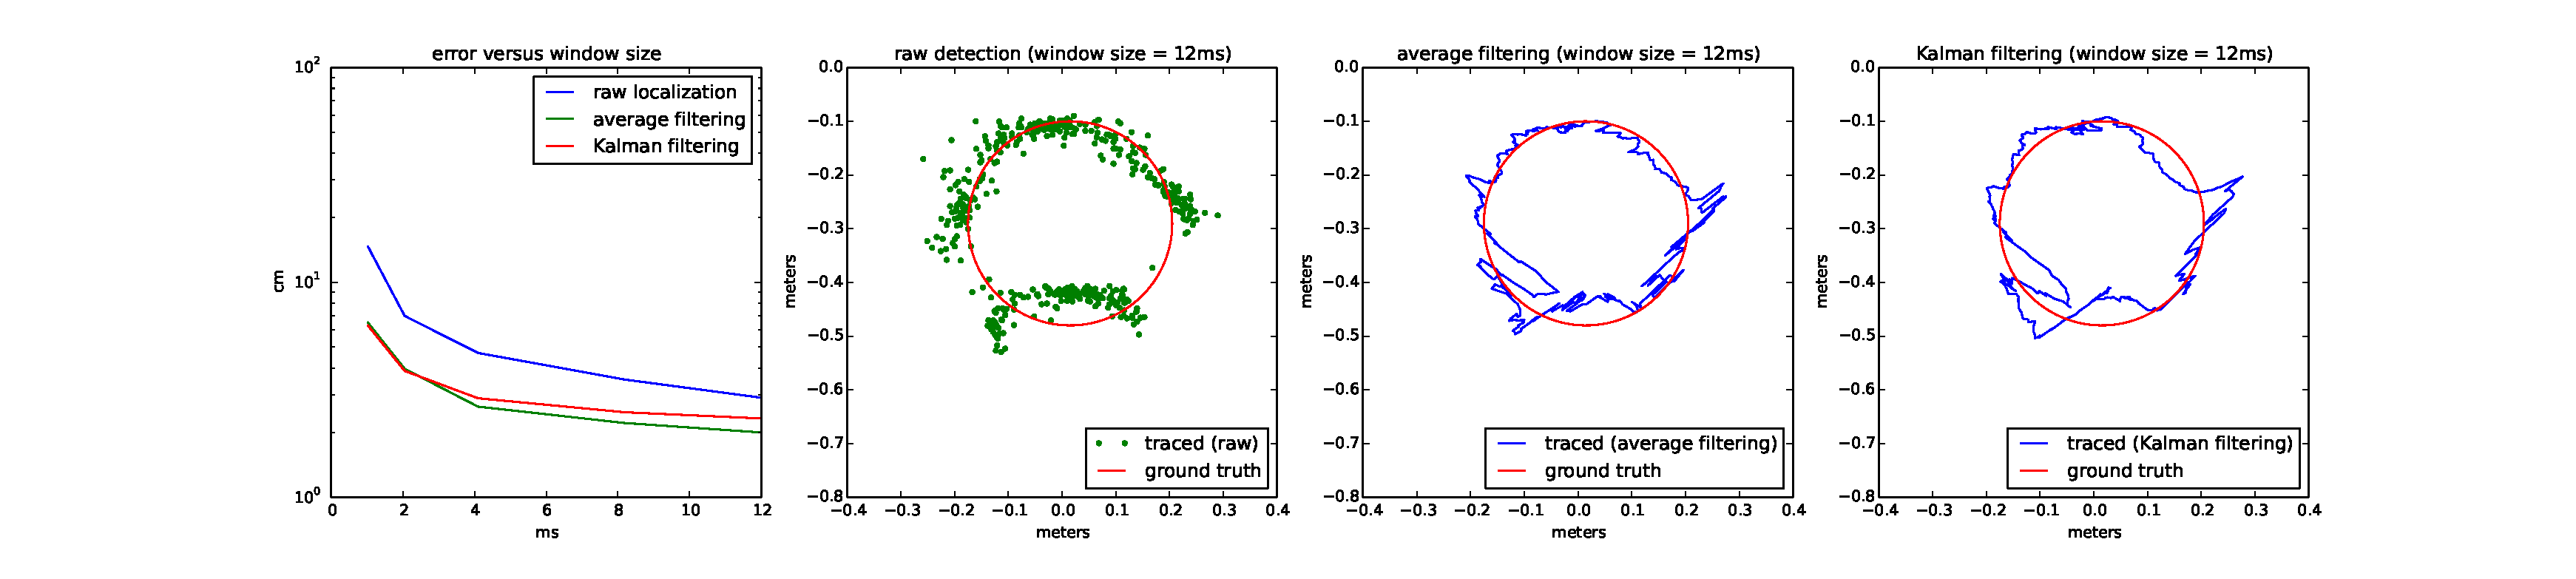
\includegraphics[width=\textwidth]{trace_output_circle_mbn.eps}
  \caption{music B}
  \label{fig:circle_musicb}
\end{subfigure}
\caption{Localization of circle movement with different sound sources. Sound source is moving at $10$ cm per second}
\label{fig:circle_normal}
\end{figure*}


Fig~\ref{fig:circle_normal} shows results for experiments with three different audio sources at normal speed.

with three different audio source were used for the same circular movement. In the first trial, white noise is used to set a baseline for audio sources, since our understanding is that white noise performs the best under GCC\_PHAT. In the second trial, a randomly picked music is used. In the third trial, a music that contains low amplitude segments is picked to reflect real life situations. Fig~\ref{fig:circle} shows the result for all three trials. From the result, white noise does perform the best and the localized shape matches well with the shape of the rotating disk. There exists a bit of jiggling, but can be improved with filtering. Fig~\ref{fig:circle} also shows the result with averaging filtering and Kalman filtering. 

For the music A, the array still localizaes correctly and the output represetns a circular shape, but the localizaed points are more spread out with more jiggling. This is because music does not have components in all frequency bands and GCC\_PHAT estimate is less accuracy with such audio sources. Similar to the white noise case, we can improve the raw tracking estimates from the array with filtering.

For music B, the music has a low amplitude section and it is also shown in the traced result. The "blank" region in the output corresponds to the low amplitude segment in the audio. The general tracking quality of this music is not as good as that with Music A due to these low amplitude audio segments. 


\begin{figure*}[]
\centering
\begin{subfigure}[]{1.0\textwidth}
  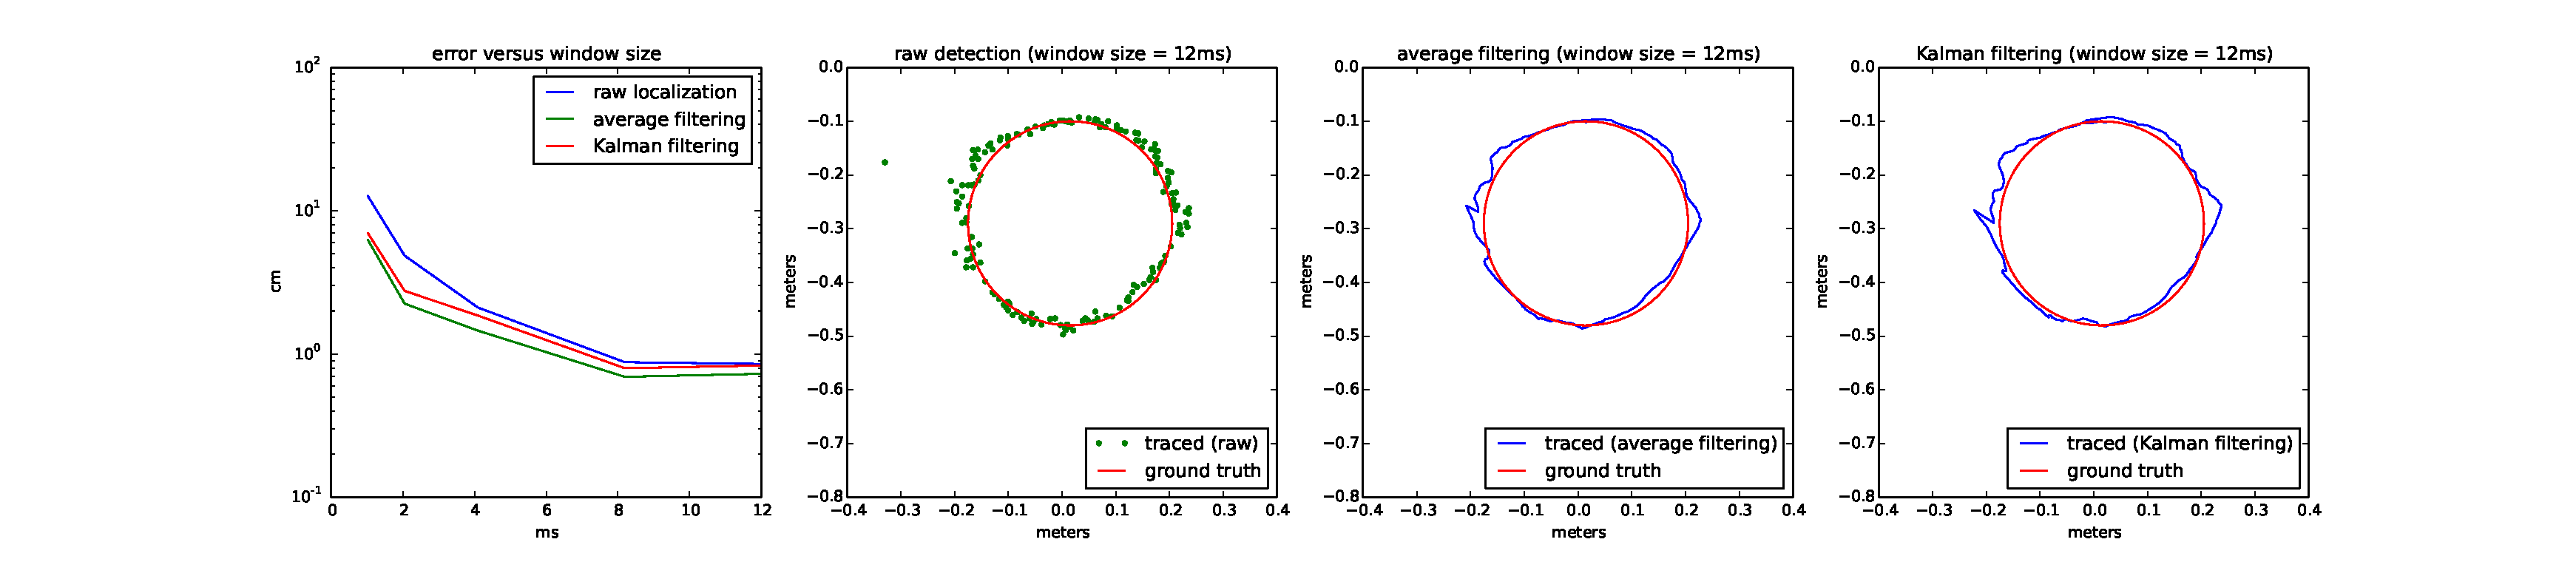
\includegraphics[width=\textwidth]{trace_output_circle_wnf.eps}
  \caption{white noise}
  \label{fig:circle_wn}
\end{subfigure}
\begin{subfigure}[]{1.0\textwidth}
  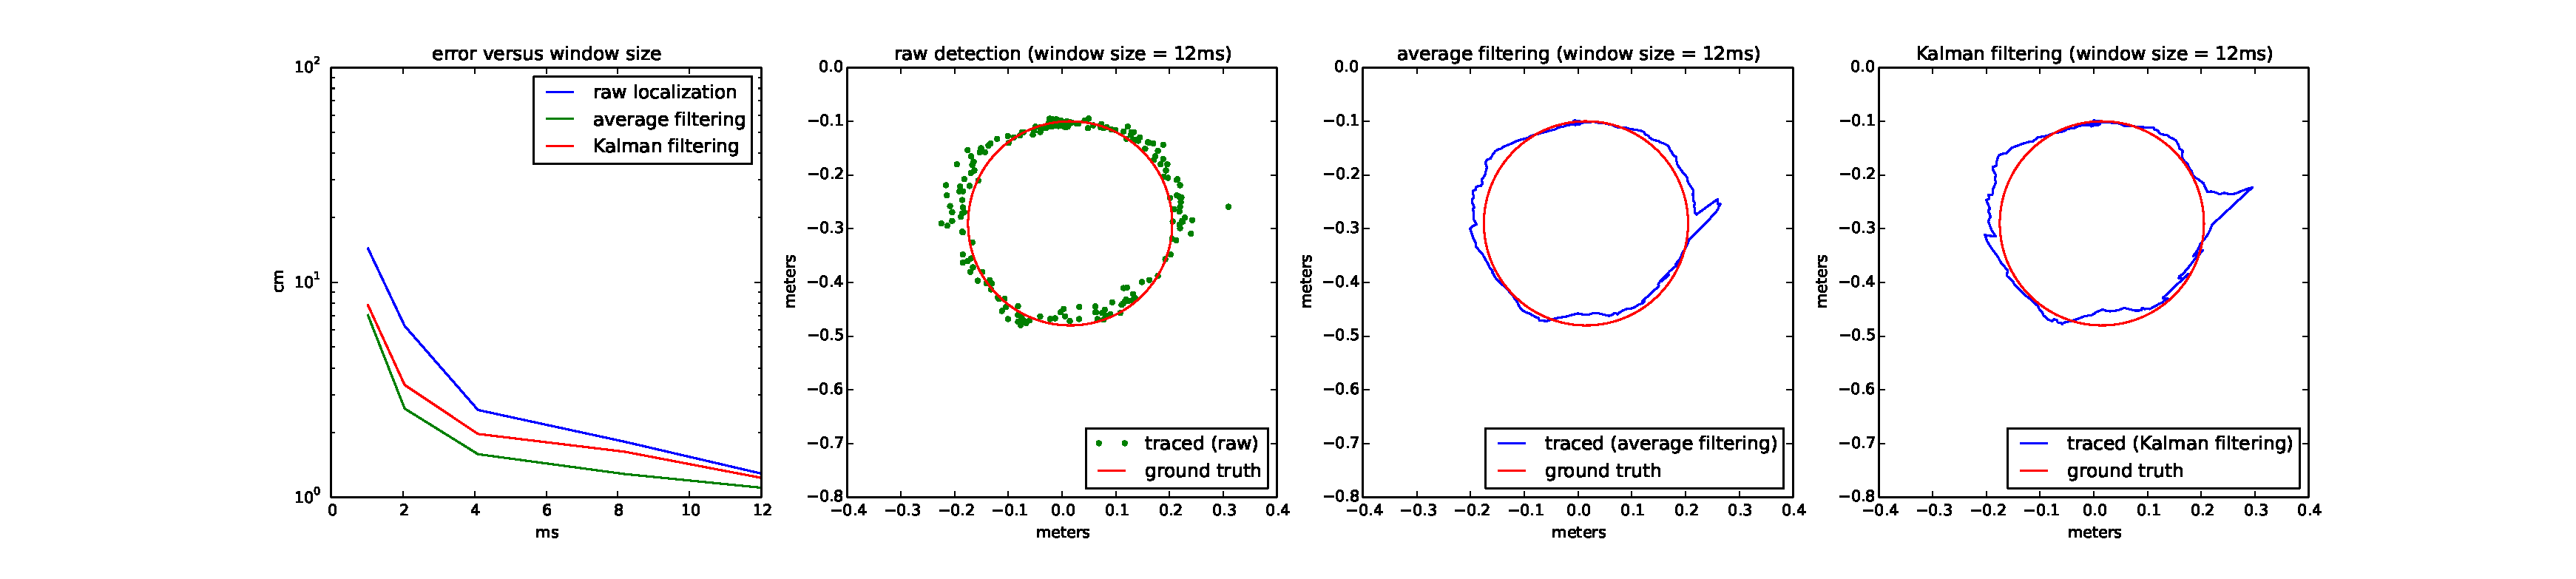
\includegraphics[width=\textwidth]{trace_output_circle_maf.eps}
  \caption{music A}
  \label{fig:circle_musica}
\end{subfigure}
\begin{subfigure}[]{1.0\textwidth}
  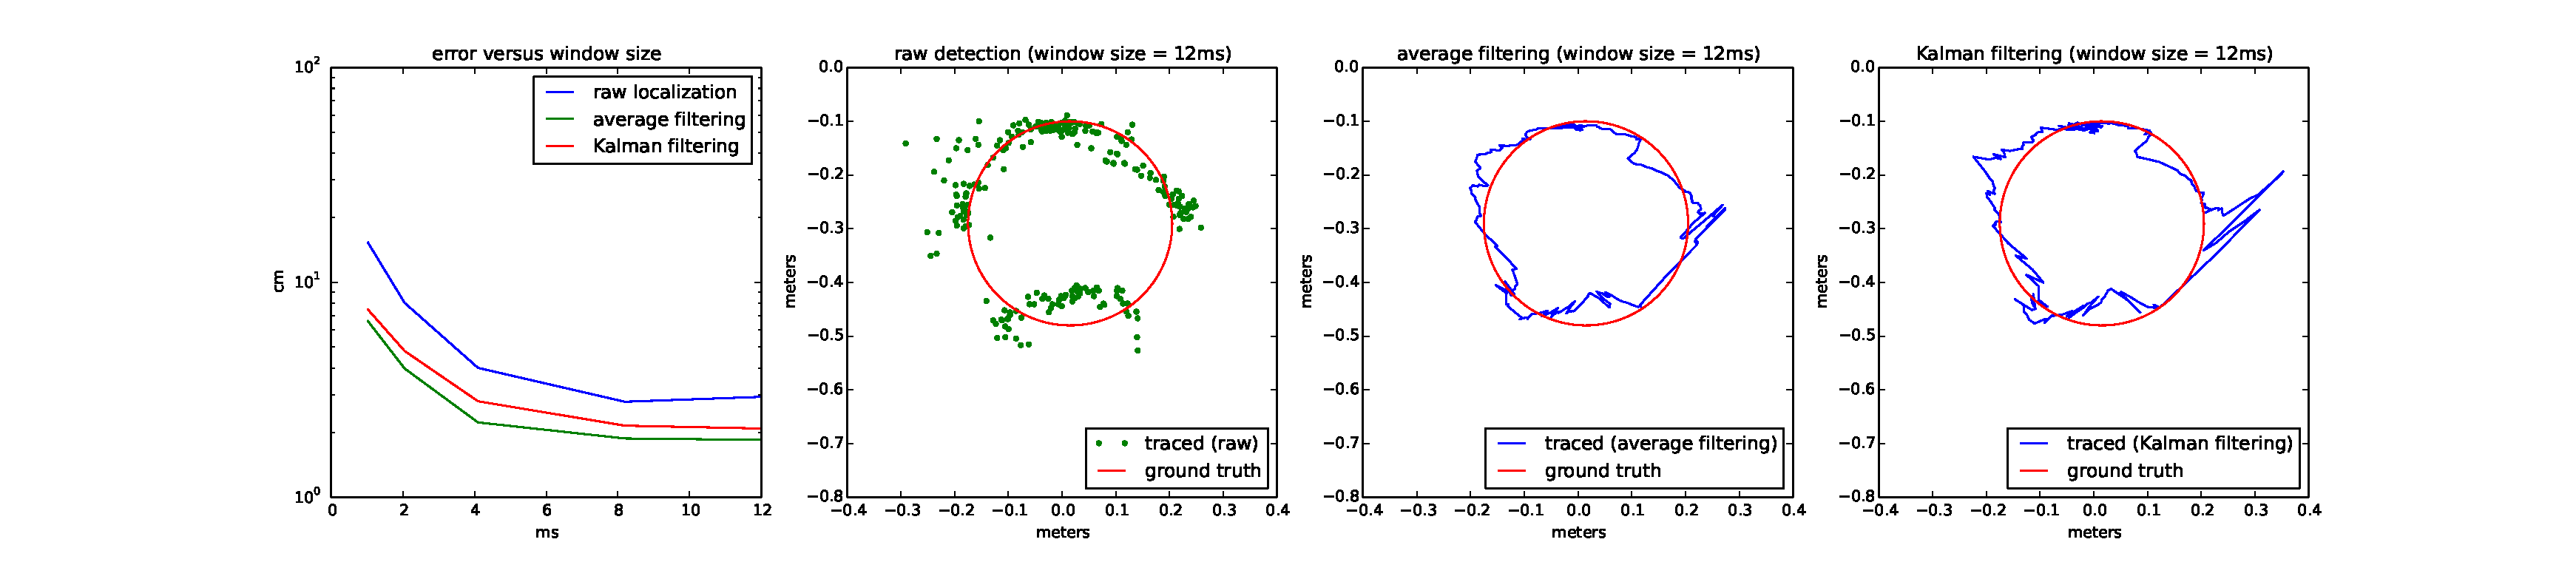
\includegraphics[width=\textwidth]{trace_output_circle_mbf.eps}
  \caption{music B}
  \label{fig:circle_musicb}
\end{subfigure}
\caption{Localization of circle movement with different sound sources. Sound source is moving at $20$ cm per second}
\label{fig:circle_fast}
\end{figure*}
